\documentclass[UTF8]{ctexart}
\usepackage{amsmath}
\usepackage{graphicx}
\usepackage{float}
\usepackage{subfigure}
\usepackage{xeCJK}
\usepackage{hyperref}
\usepackage{algorithm2e}
\usepackage{amsfonts}
\usepackage{epsfig}
\usepackage{listings}
\usepackage{xcolor}
% 定义可能使用到的颜色

\definecolor{CPPLight}  {HTML} {686868}
\definecolor{CPPSteel}  {HTML} {888888}
\definecolor{CPPDark}   {HTML} {262626}
\definecolor{CPPBlue}   {HTML} {4172A3}
\definecolor{CPPGreen}  {HTML} {487818}
\definecolor{CPPBrown}  {HTML} {A07040}
\definecolor{CPPRed}    {HTML} {AD4D3A}
\definecolor{CPPViolet} {HTML} {7040A0}
\definecolor{CPPGray}  {HTML} {B8B8B8}
\lstset{
    columns=fixed,
    numbers=left,                                        % 在左侧显示行号
    frame=none,                                          % 不显示背景边框
    backgroundcolor=\color[RGB]{245,245,244},            % 设定背景颜色
    keywordstyle=\color[RGB]{40,40,255},                 % 设定关键字颜色
    numberstyle=\footnotesize\color{darkgray},           % 设定行号格式
    commentstyle=\it\color[RGB]{0,96,96},                % 设置代码注释的格式
    stringstyle=\rmfamily\slshape\color[RGB]{128,0,0},   % 设置字符串格式
    showstringspaces=false,                              % 不显示字符串中的空格
    language=c++,                                        % 设置语言
    morekeywords={alignas,continute,friend,register,true,alignof,decltype,goto,
    reinterpret_cast,try,asm,defult,if,return,typedef,auto,delete,inline,short,
    typeid,bool,do,int,signed,typename,break,double,long,sizeof,union,case,
    dynamic_cast,mutable,static,unsigned,catch,else,namespace,static_assert,using,
    char,enum,new,static_cast,virtual,char16_t,char32_t,explict,noexcept,struct,
    void,export,nullptr,switch,volatile,class,extern,operator,template,wchar_t,
    const,false,private,this,while,constexpr,float,protected,thread_local,
    const_cast,for,public,throw,std},
}

\graphicspath{{images/}}
\setCJKmonofont{Microsoft YaHei}

\title{\Huge{计算机算法设计与分析\\ 分支限界法}}
\author{\Huge{易凯}}
\date{\Huge{2017年5月24日}}

\begin{document}
    \maketitle
    \vspace{35mm}
    \begin{flushright}
    \Large{
    \textbf{班\ \ \ \ \ 级} \makebox[5em][l]{软件53班}

    \textbf{学\ \ \ \ \ 号} \makebox[5em][l]{2151601053}

    \textbf{邮\ \ \ \ \ 箱} \makebox[5em][l]{williamyi96@gmail.com}

    \textbf{联系电话} \makebox[5em][l]{13772103675}

    \textbf{个人网站} \makebox[5em][l]{https://williamyi96.github.io}

                      \makebox[5em][l]{williamyi.tech}

      \textbf{实验日期} \makebox[5em][l]{2017年5月24日}

    \textbf{提交日期} \makebox[5em][l]{2017年6月6日}
    }
    \end{flushright}

    \newpage
  	\tableofcontents
  	\newpage
  	\listoffigures
    \newpage

    \section{分支限界法与回溯法基本区别}
    \subsection{求解目标不同}
    回溯法的求解目标是找出解空间中满足约束条件的所有解,而分支限界法的求解目标则是找出满足约束条件的一个解或者是某种意义上的最优解。

    \subsection{搜索方式不同}
    回溯法采用深度优先的方式对解空间进行搜索,而分支限界法采用广度优先或者是最小耗费优先的方式进行搜索。

    \section{分支限界法实现方式}
    分支限界法根据从活结点表中选择下一个扩展结点的不同方式从而派生出了分支限界法的两种不同实现方式。其分别为队列式分支限界法和优先队列式分支限界法。

    \subsection{队列式分支限界法}
    队列式分支限界法就是将活结点表排成一个队列,按照队列的先进先出原则选择下一个结点为当前的扩展结点。
    \subsection{优先队列式分支限界法}
    优先队列式的分支限界法将活结点表组织成一个优先队列,并按照优先队列中规定的结点优先级选取优先级最高的下一个结点成为当前扩展结点。

    \section{栈式分支限界法和回溯法的区别}
    \subsection{题目描述}
    栈式分支限界法将活结点表以LIFO(后进先出)的方式存储在一个栈中。试设计一个解0-1背包问题的栈式分支限界法,并说明栈式分支限界法和回溯法之间的区别。
    \subsection{题目解答}
    该算法的基本思想较为清晰,具体的代码如下:

    \begin{small}
    \begin{lstlisting}
    template<class Typew, class Typep>
    Typep Knap<Typew, Typep>::StackKnapsack() {
        //栈式分支限界法,返回最大的价值,同时定义栈的容量初始化为10000
        S = new Stack<HeapNode<Typep, Typew>>(10000);
        int i = 1, e = 0, cw = cp = 0;
        //e为当前的扩展结点,cw为该结点对应的重量,cp表示的是相应的价值,up是价值上界。
        Typep bestp = 0; //bestp 为当前最优值;
        Typep up = Bound(1); //up为价值上界
        //进行子集空间树搜索
        while(1) {
            //检查当前扩展结点的左儿子结点
            Typew wt = cw + w[i]
            if(wt <= c) {
                //左儿子结点为可行结点
                if(cp + p[i] > bestp) bestp = cp + p[i];
                AddLiveNode(up, cp + p[i], cw + w[i], true, i+1);
            }
            up = Bound(i+1);
            //检查当前扩展结点的右儿子结点
            if(up >= bestp) //右子树可能含有最优解
                AddLiveNode(up, cp, cw, false, i+1);
            //取下一扩展结点
            if(S->empty()) return bestp;
            HeapNode<Typep, Typew> H;
            S -> pop(H);
            e = H.ptr;
            cw = H.weight;
            cp = H.profit;
            up = H.upprofit;
            i = H.level;
        }
    }
    \end{lstlisting}
    \end{small}
    然后通过上述方式进行结点的使用即可,其中后续的部分与有限队列式分支限界法大致相同。在此不进行赘述。
    \subsection{栈式分支限界法与回溯法的区别}
    根据其名称上来看,我们就可以得到栈式分支限界法与回溯法的最大区别就是分支限界法和回溯法的区别,而其主要是对于当前扩展结点所采用的扩展方式不同。在分支限界法中,每一个活结点只有一次机会成为扩展结点。活结点一旦成为扩展结点,就一次性产生其所有儿子结点。在这些儿子结点中将不可行的解进行舍弃,然后再将可行的儿子结点加入表中。那些在或结点表中的结点然后依据栈的特点逐个取出相应结点,使其成为扩展结点,重复上述过程知道找到最优解。而由于回溯法使用的是深度优先策略,则其每个结点可能多次成为活结点。

    \section{修改MaxLoading}
    \subsection{题目描述}
    修改解装载问题的分支限界算法MaxLoading,使得算法在结束前释放所有已由EnQueue产生的结点
    \subsection{题目求解}
    \begin{small}
    \begin{lstlisting}

    以下仅说明主要更改的部分:
    while(1) {
        Type wt = ew - w[i];
        if(wt <= c) {//结点可选
            if(wt > bestw) bestw = wt;
            EnQueue(Q, wt, i, n, bestw, e, beste, bestx, true);
        }
    }
    \end{lstlisting}
    \end{small}

    \section{旅行售货员分支限界法的修改}
    \subsection{题目描述}
    试修改解旅行售货员问题的分支限界法,使得算法保存已产生的排列树。
    \subsection{问题求解}
    remain to be seen.

    \section{无优先级运算问题}
    \subsection{问题描述}
    给定n个正整数和4个运算符+,-,*,/,且运算符无优先级,如2+3*5=25。对于任意给定的整数m,是设计一个算法,用以上给出的n个数和4个运算符,产生整数m,且用的运算次数最少。给出的n个树中的每个数最多只能用1次,但每种运算符可以任意使用。
    \subsection{算法设计}
    对于给定的n个整数,采用回溯方法来设计一个算法,用最少的无优先级运算次数产生整数m。
    \subsection{数据输入}
    输入的第一行有两个正整数n和m,第二行是给定的用于运算的n个正整数。
    \subsection{结果输出}
    将计算的产生整数m的最少无优先级计算次数以及最优无优先级表达式输出到屏幕上。
    \subsection{程序代码}
    \begin{small}
    \begin{lstlisting}
#include<iostream>
using namespace std;

int k;
class readin {
	friend int nreadin(int n,int m);
private:
	bool found();                  //found判断是否找到解
	bool search(int t);
	int n,m,x;
    int* a;                        //给定的用于运算的n个正整数的存放位置
	int* num;                      //存放运算的产生整数m
	int* operate;
	int* flag;
	char* ptr;                     //存储结果中的运算符
};

bool readin::search(int depth)  {
	if(depth>k) {
		if(found())
			return true;           //判断结点是否满足条件,即是否找到解
		else
			return false;
	}
	else
		for(int i=0;i<n;i++)
			if(flag[i]==0){
				num[depth]=a[i];
				flag[i]=1;
				for(int j=0;j<4;j++){
					operate[depth]=j;
					if(search(depth+1))
						return true;
				}
				flag[i]=0;
			}
			return false;
}

bool readin::found(){
	int x=num[0];
	for(int i=0;i<k;i++){
		switch (operate[i]){
		case 0:x+=num[i+1];ptr[i]='+';break;
		case 1:x-=num[i+1];ptr[i]='-';break;
		case 2:x*=num[i+1];ptr[i]='*';break;
		case 3:x/=num[i+1];ptr[i]='/';break;
		}
	}
	return(x==m);
}

//读入初始数据
int nreadin(int n,int m){
	readin X;
	int* a=new int[n];
    int* num=new int[n];
    int* operate=new int[n];
    int* flag=new int[n];
	char* ptr=new char[n];
	X.n=n;
	X.m=m;
	X.a=a;
	X.operate=operate;
	X.flag=flag;
	X.num=num;
	X.ptr=ptr;
	for(int i=0;i<n;i++)
{
		cin>>a[i];
		flag[i]=0;
	}
	for(k=0;k<n;k++)
		if(X.search(0)){
	        cout<<k<<endl;
	        for(int i=0;i<=k;i++){
				cout<<num[i]<<ptr[i];
			}
			cout<<endl;
			return 0;
		}
		return 0;
}

int main(){
	int n;
    int m;
	cin>>n>>m;
    nreadin(n,m);	
    return 0;
}
    \end{lstlisting}
    \end{small}
    \subsection{样例运行}
    \begin{figure}[!htb]
      \centering
      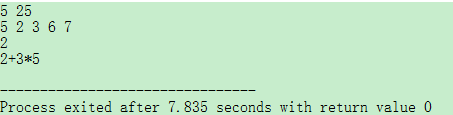
\includegraphics[width=0.6\textwidth]{../img/6.9.PNG}
      \caption{无优先级问题样例运行}\label{无优先级问题样例运行}
    \end{figure}
\end{document} 